\chapter{Study Case} \label{chap:robi}

This thesis was proposed as part of a robotic agriculture project which consists in the development of a mobile manipulator for agricultural applications called ROBI'. In this chapter we will explain the main characteristics of the project, focusing in the electronic architecture and in the systems that should be controlled by the motor driver developed in this thesis. The information for this chapter was obtained from \citeauthor{robi:2017} \citetitle{robi:2017} \citeyear{robi:2017} and from \citeauthor{robi2:2017} \citetitle{robi2:2017} \citeyear{robi2:2017}.

\section{Robi}

ROBI' is a mobile manipulator for agricultural applications. The development of this project has the objective of becoming a platform for research, development and testing of different perception and control algorithms. The robot was designed following low-cost, low-weight, simplicity, flexibility and modularity requirements, in order to allow an easy implementation of the work developed as part of this project.

\begin{figure}[htbp]
\centering
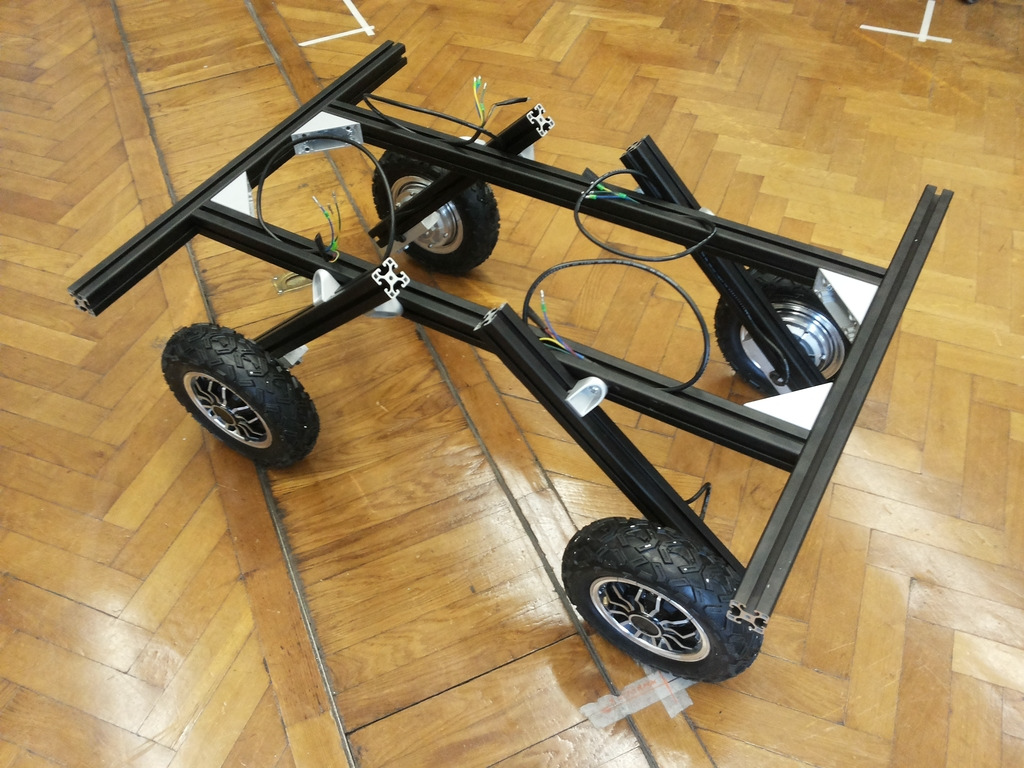
\includegraphics[width=10cm]{Images/robi.png} 
\caption[ROBI' Basic Configuration]{ROBI' Basic Configuration}
\label{fig:robi_picture}
\end{figure}

\section{In-Wheel Motors}

One of the most important components of ROBI' for this thesis is the in-wheel motor system used as motor drive. As mentioned in the introduction, in-wheel motors have the advantage that there is no need for an external power transmission mechanism, due to the fact that the motor is embedded into the wheel. This also reduces the space needed for the motor drive system, as well as the weight of the robot, increasing the payload capacity of the electric motor.

It is also interesting to mention that this configuration of the drive system allows the control of each one of the wheels of the robot independently, which allows the implementation of different control methods for this robot, like skid steering, which relies on the slip effect of the wheels in the terrain and requires a good control of the torque and the speed of each one of the motors.

\begin{table}[]
\centering
\caption{HUB10GL in-wheel motor main characteristics}
\label{table:hub10}
\begin{tabular}{@{}ll@{}}
\toprule
Motor mass                & 3.5 kg   \\
Motor and tire mass       & 5.7 kg   \\
Tire diameter             & 254 mm   \\ 
Power                     & 500 W    \\
Voltage                   & 36 V     \\
Maximum speed             & 1350 RPM \\
Phase-to-phase resistance & 160 m$\Omega$\\
Phase-to-phase inductance & 0.76 mH \\
Pole Pairs				  & 10		\\
$K_{E}$					  & 0.36 V/(rad/s) \\
$K_{T}$					  & 0.4506 Nm/A \\
\bottomrule
\end{tabular}
\end{table}

The in-wheel motor installed in the robot is a \ac{PMSM} motor and its main characteristics are mentioned in Table \ref{table:hub10}. 

In order to take advantage of the sinusoidal distribution of the windings of this motor, an absolute angular position sensor was installed in the drive system in order to be able to apply a \ac{FOC} loop. The sensor was attached to the wheel by means of a toothed pulley system in order to keep it away from the ground.

\begin{figure}[htbp]
\centering
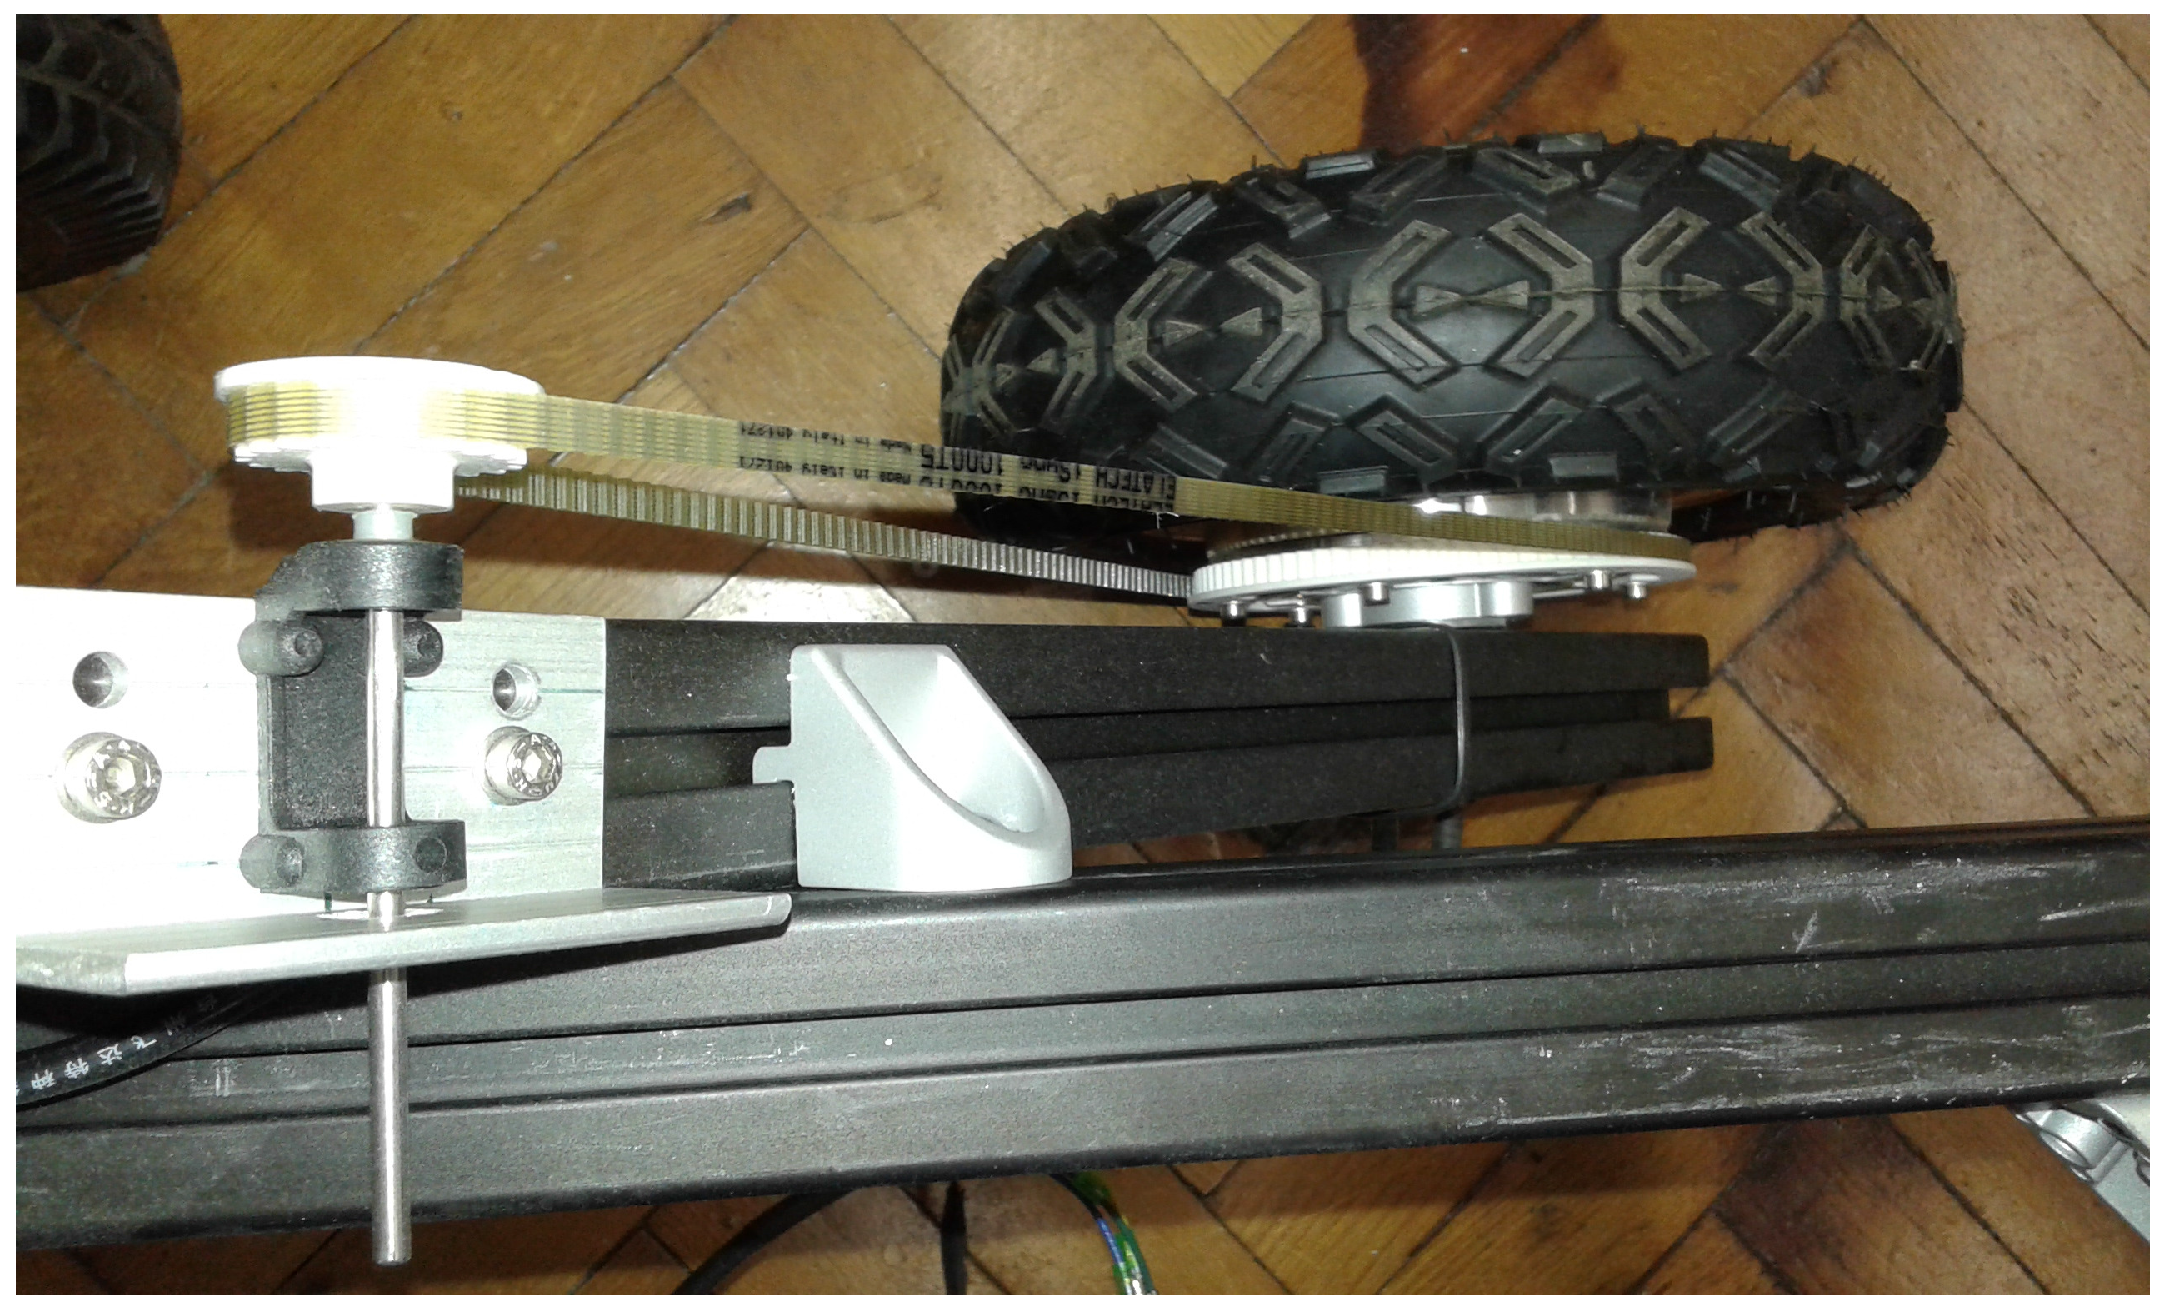
\includegraphics[width=10cm]{Images/orbis_pulley.png} 
\caption[Encoder Transmission Configuration]{Encoder transmission configuration}
\label{fig:orbis_pulley}
\end{figure}

The angular position sensor used is an Orbis encoder, manufactured by RLS. As mentioned in \ref{subsection:angular_sensors}, this is a magnetic encoder which works by reading the orientation of the magnetic field of a permanent magnet attached to a shaft. The encoder has a resolution of 14 bits with a sensitivity of $\pm0.3$\degree and transmits the angular position information through a modified \acf{SPI} called \acf{SSI}, which sends the 14 bits in \ac{SPI} slave write-only mode through a RS422 transceiver. 

In this case, the shaft is not directly the shaft of the rotor, but it's the shaft of the pulley system. This transmission system has a 4.6 size ratio due to the space constraints of the system. As mentioned in \ref{subsection:angular_sensors}, this motor includes three Hall effect sensors, even if it's a \ac{PMSM} motor.

\section{Power Architecture}

Another importan aspect for the development of this work is the power supply. In the case of ROBI', the power supply consists on three $12V$ lead acid deep-cycle batteries connected in series to provide $36V$ to the different components of the robot.

\begin{table}[]
\centering
\caption{Battery main characteristics}
\label{table:battery}
\begin{tabular}{@{}ll@{}}
\toprule
Manufacturer	&	FIAM				\\
Model			&	FGC22703			\\
Type			&	Sealed lead acid 	\\
Voltage			&	12 V 				\\
Capacity 		&  	27 Ah 				\\
\bottomrule
\end{tabular}
\end{table}

\section{Electronic Architecture}

It is important to understand the expected electronic architecture in order to consider the peripherals that the microcontroller has to include to communicate with the rest of the systems inside the robot.

The electronic architecture of ROBI' was designed to be similar to an automotive \acf{ECU} based system. In this architectures, all the \ac{ECU}s interact with each other through a communication bus called \acf{CAN}.

\begin{figure}[htbp]
\centering
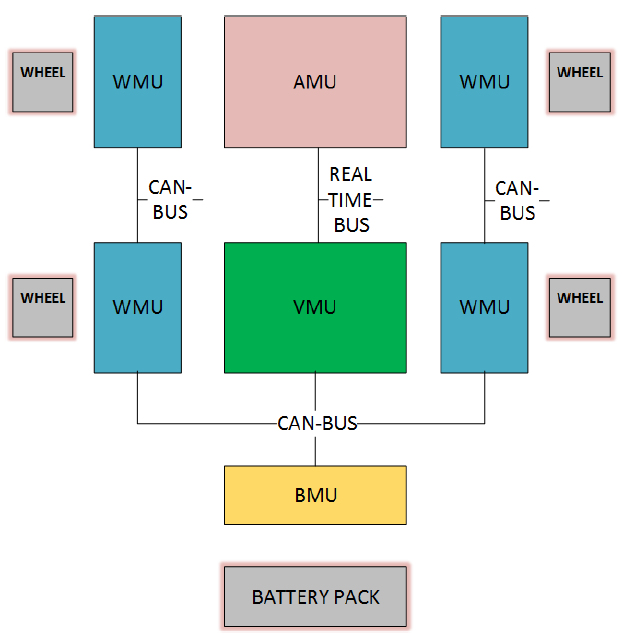
\includegraphics[width=10cm]{Images/ecus.png} 
\caption[ECUs architecture]{ECUs architecture: functional block diagram}
\label{fig:ecus}
\end{figure}

As it can be seen in Figure \ref{fig:ecus}, the \ac{ECU}s network consists on four units: \acf{WMU}, \acf{BMU}, \acf{VMU} and \acf{AMU}. The one that is being developed here is the \ac{WMU}, and it will be described in the following chapters.